\section{Introduction to Online Advertising}

In online advertising, advertisers distribute promotional marketing messages to potential consumers through the Internet. Already a multi-billion dollar industry, online advertising is still showing rapid growth. This growth in the online advertising industry is attributed to multiple factors including considerably cheap and more targeted advertising compared to its offline counterparts, world wide coverage of the Internet, the velocity of ad delivery and quick feedback mechanisms.



\subsection{History of Online Advertising}
The notion of online advertising started in 1994 with the first clickable ad by Wired magazine's online counterpart, HotWired. HotWired devised a plan to set aside portions of its website to sell space to advertisers, similar to how ad space is sold in a print magazine. That is how banner advertising was born. Banner advertising quickly grew as a prominent method for websites to keep their content ungated and free for users. In 1995, ad servers were introduced and the concept of targeting relevant websites was started. Multiple services started operating which would help advertisers select websites where they could potentially find the desired consumer demographics. Around 1998, ad networks were formed and user targeting started becoming more prominent.

With search engines steadily gaining popularity in late 90s, following years also saw the rise of search engine advertising. Advertisers who were looking to create ads that were more targeted turned to sponsored search. Initially Paid Placement Model (PPM) was offered for search engine advertising where an advertiser would directly bid upon the keywords and based solely on the bid, the ad slot would be assigned. Google modified PPM by emphasizing more on user experience and hence, an ad's position on the query results page was determined by not only the bid of the advertiser but also by the relevance of the ad to the query and other features like Click-Through-Rate. 


The next break-through came into display advertising. Around 2007, demand side and supply side platforms were introduced where the idea of Real Time Bidding (RTB) was put forward. RTB allows advertisers to bid in real time for incoming ad slots. The bidding is usually done automatically but can also be done manually. RTB allowed advertisers to be more specific with respect to the targeted potential consumers and at the same time, it allowed publishers to sell most of the ad space as one impression is sold at a time.

Meanwhile, the social media ecosystem started developing around early 2000s with the advent of LinkedIn and Facebook and social media advertising started around 2005. Facebook allowed user level targeting and was a unique player in the market to accurately target demographics. Social media advertising later advanced to sponsored posts. Very recently, Facebook also started mobile ads on its mobile applications in order to target consumers in real time based on the location and other hyper-demographics.

%\begin{figure}
%	\centering
%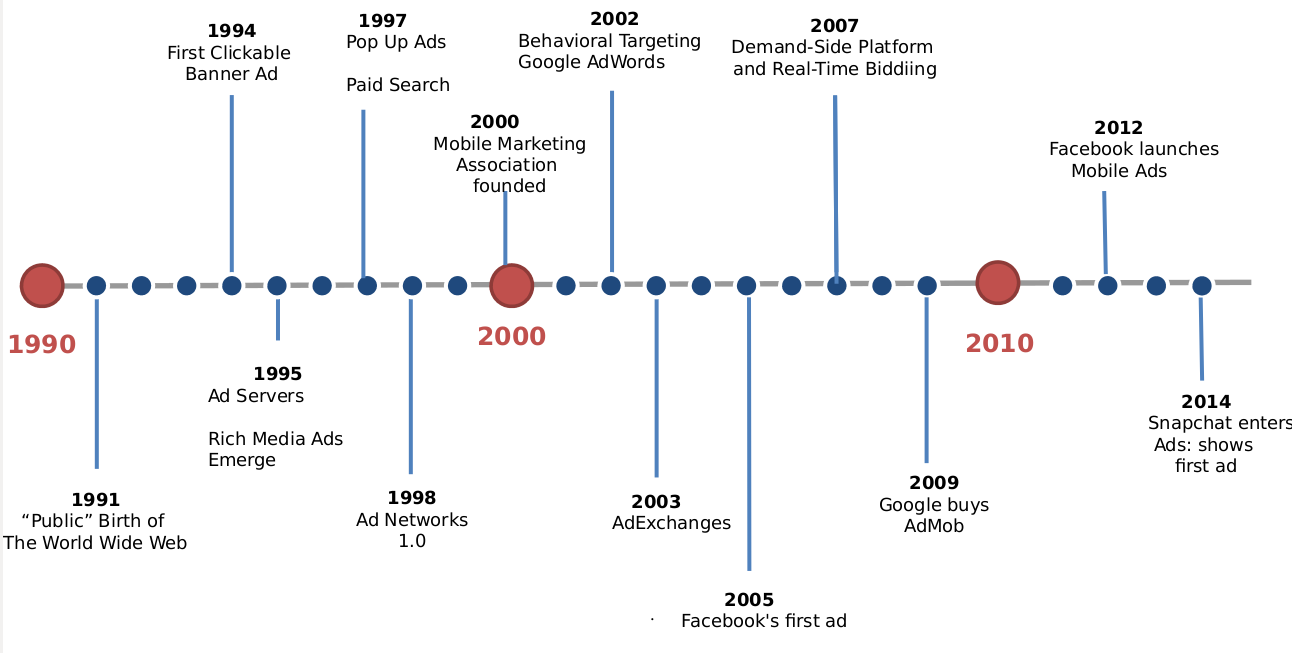
\includegraphics[scale=0.34]{visuals/history.png}
%	\caption{Major events in the online advertising landscape}
%	\label{fig:events}
%\end{figure}




Aside from the Internet explosion, the mobile era was steadily developing since early 90s. Around 2000, the Mobile Marketing Association was founded for the development of mobile ads and the first SMS ad was served in the same year by a Finnish news provider by offering free news headlines sponsored by advertising. This initiative also led to other experiments in mobile marketing and with the advent of smart phones in late 2000s, mobile advertising started growing at a very accelerated rate.  Now, mobile advertising includes all forms of web advertising including sponsored search and banner ads. 



The current status of online advertising is targeting `potential' consumers who would make a transaction and not just click the ad. In order to achieve this, almost all players in the market are trying to achieve behavioral targeting at a very granular level by employing multiple data sources like chat logs, social media activities, local information, etc. A key role in behavioral targeting is played by mobile phones as they are a real time source of user activity. In fact, in the latest report by Internet Advertising Bureau (IAB), they state that mobile advertising has the highest growth in revenue in the past decade \cite{IAB2016}.

%\begin{figure}
%	\centering
%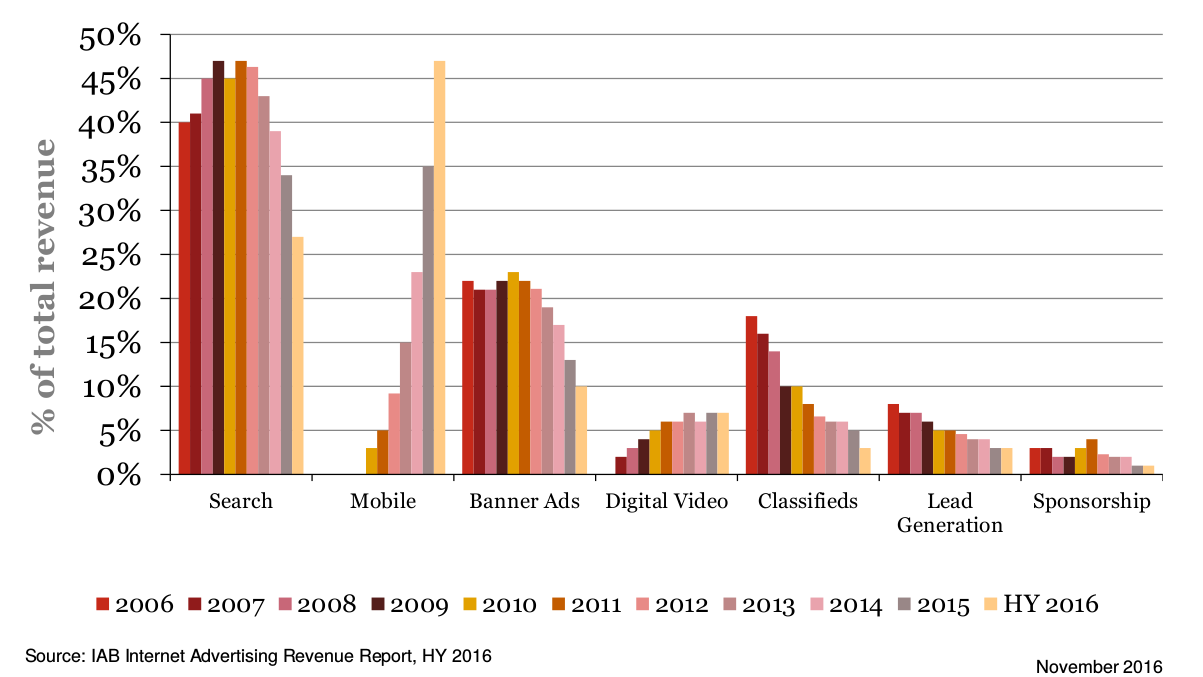
\includegraphics[scale=0.35]{visuals/IABReport.png}
%	\caption{Historical trends in internet advertising formats Revenue share by major ad formats \cite{IAB2016}}
%	\label{fig:history}
%\end{figure}



\subsection{Types of Online Advertising}

Based mechanism of delivery, online advertising is classified into the following categories - \textit{Display Advertising}, \textit{Social Media Advertising}, \textit{Sponsored Search}, \textit{Email advertising} and \textit{Online Classified Ads}. 


\subsubsection{Display Advertising}
Display advertising is the graphical information that appears next to content on web pages. This can include rich content beyond text such as logos, pictures and even videos. In display advertising, advertisers can either opt for guaranteed contracts (i.e. the publisher will show the number of ads as determined by the contract for a fixed price) or real time bidding (i.e. where each impression is sold individually via auctions through ad servers). Display advertising can be further classified into pop-up ads and banner ads. Pop-up are generally same as banner ads except they pop-up on the screen suddenly to grab attention.


\begin{figure}
	\centering
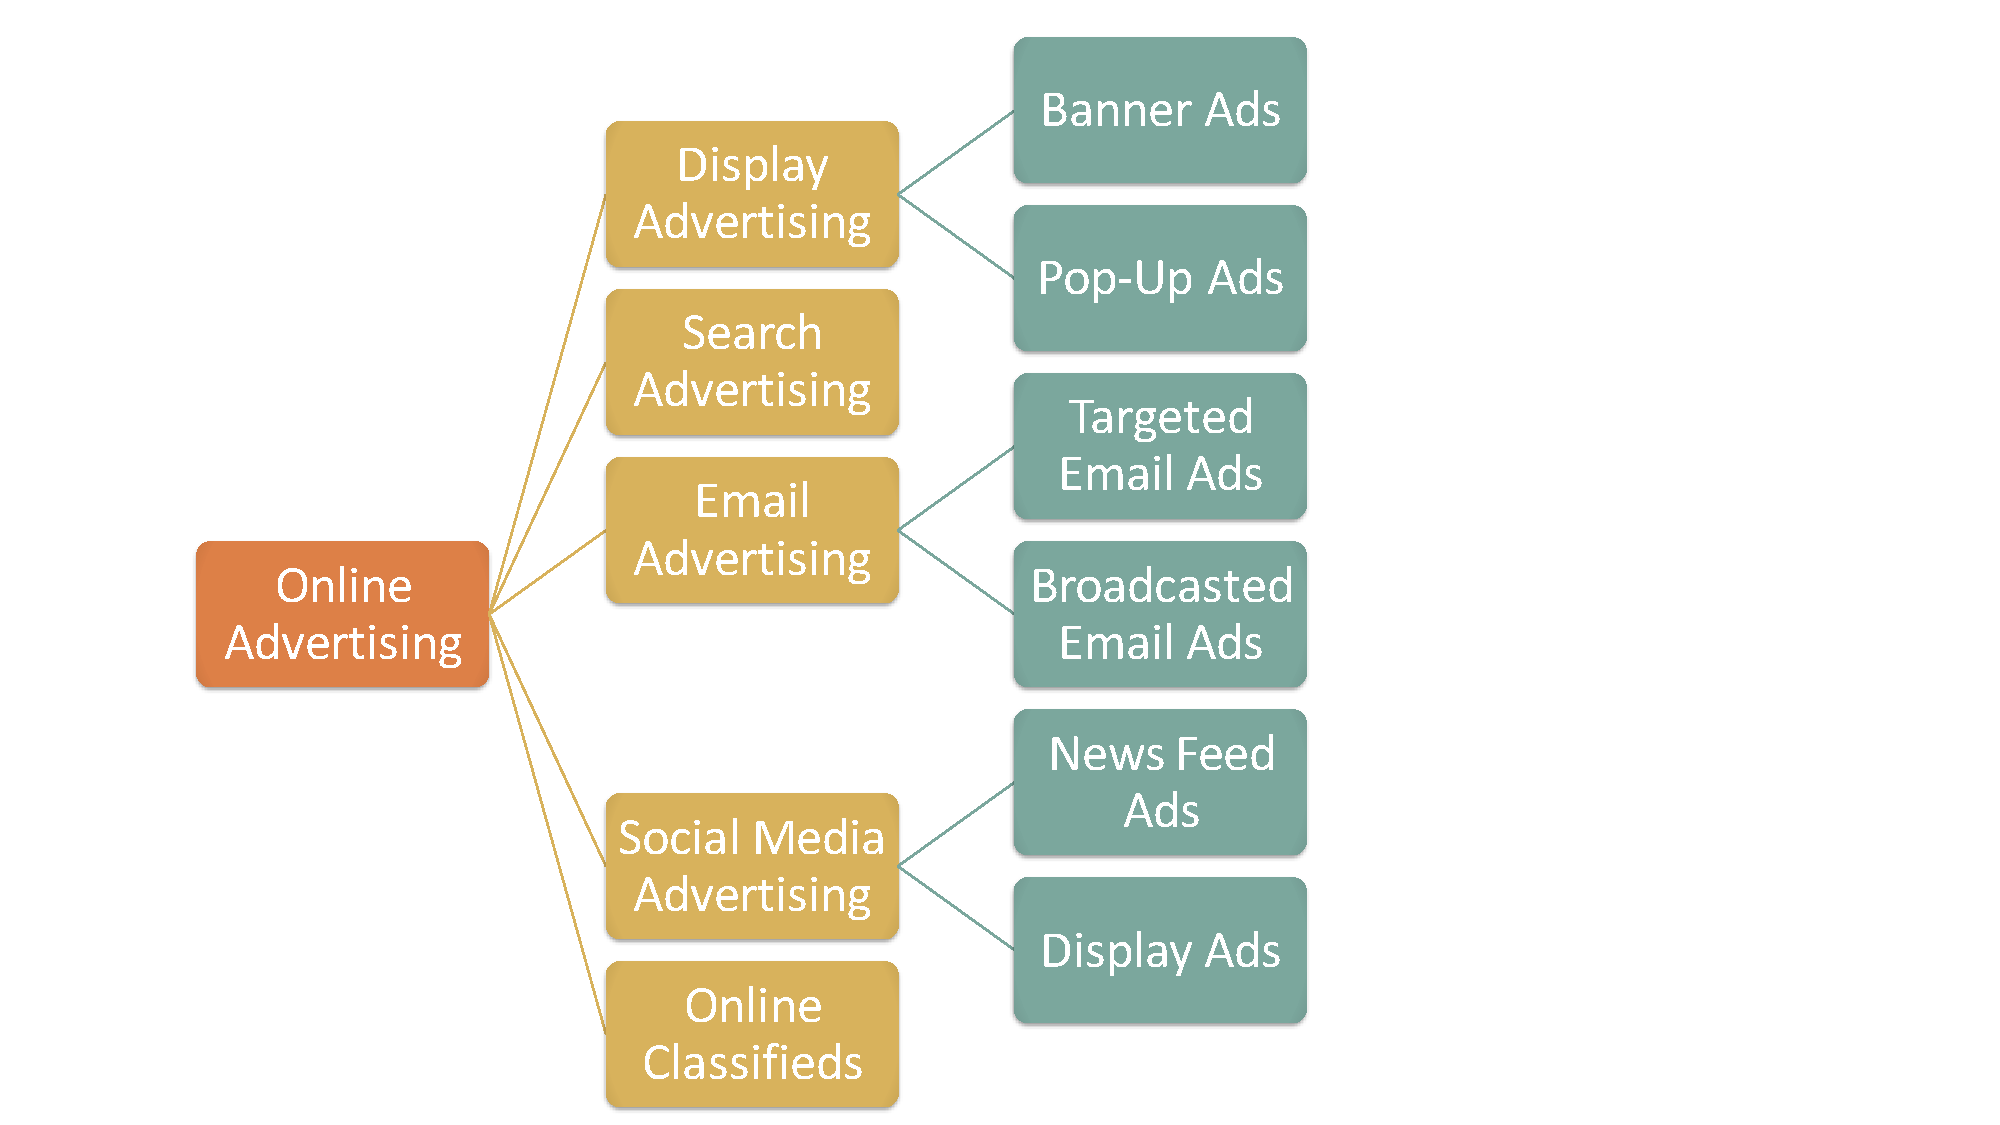
\includegraphics[scale=0.5]{visuals/Presentation.pdf}
	\caption{Types of Online Advertising based on mechanims of delivery}
	\label{fig:types}
\end{figure}


\subsubsection{Social Media Advertising}

Social media advertising has been defined as ``any piece of online content designed with a persuasive intent and distributed through social media which enables the users to access, share and engage with it'' \cite{alhabash2017social}. Social media advertising can also be further classified into two types: news feed ads and display ads.
News feed ads are the ads that are incorporated along with organic content in the news feed of the users. These are also popularly known as `sponsored posts'. Display ads in social media are the ones which are shown outside the news feed, such as on the right side of Facebook.




\subsubsection{Sponsored Search}
Sponsored search refers to advertising on search engines. When a user poses a query to the search engine, ads are shown along with the search results. Search advertising is referred to as sponsored search because advertisers have to pay to be displayed on the search results page whereas organic content is freely displayed. Figure \ref{fig:ss_example} shows a snapshot of search results containing ads and organic content.

In the next section, sponsored search will be discussed in more detail as this thesis contributes to long tail advertising in sponsored search.
 



\subsubsection{Email Advertising}
Email advertising refers to sending a commercial message to one or more potential customers. Email advertising generally involves catchy subjects and rich media to attract costumers. Generally, the goal of email advertising is to build loyalty, trust, or brand awareness. Email advertising can also be further classified into targeted email advertising and broadcast email advertising.


In targeted email advertising, promotions are sent to only specific a set of people who match the advertiser's criteria whereas in broadcast email marketing, emails are sent to everyone whose address is present in the email database.

\subsubsection{Online Classified Ads}

Online classified ads are ads which are posted online in categorical listings. Examples include online yellow pages and job portals. Quickr and Craigslist are some of the most prominent online classified ad providers.


\begin{figure}
	\centering
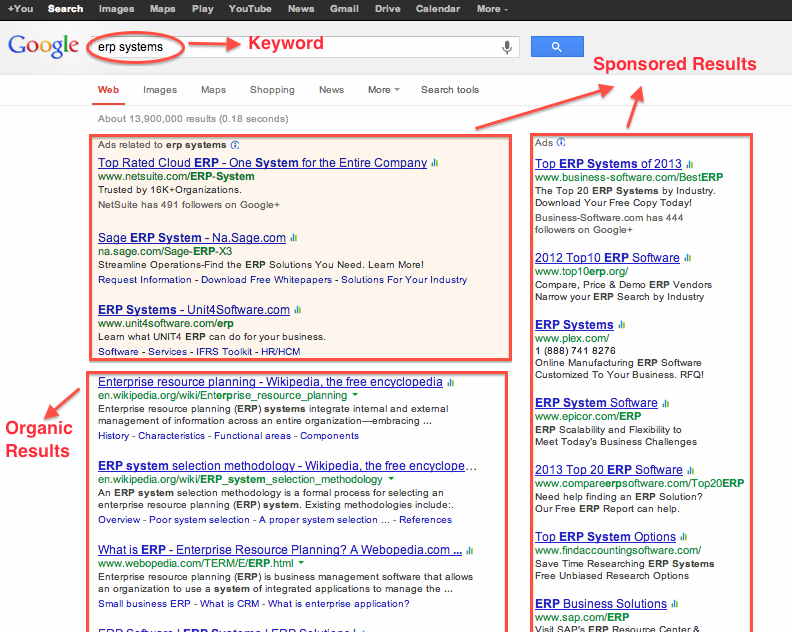
\includegraphics[scale=0.4]{visuals/ss_example.png}
	\caption{Example of query's results page from Google showing sponsored search results}
	\label{fig:ss_example}
\end{figure}


\section{Sponsored Search}

The model of search engine advertising is more popularly known as sponsored search. When a user poses a query to the search engine, ads are shown along with organic search results. Figure \ref{fig:ss_example} shows a snapshot of sponsored search from Google.


In sponsored search, advertisers bid upon search keywords which they deem relevant to their product. When a user queries the search engine, all the advertisers who chose to bid upon the keywords contained in query are considered as candidate advertisers to be shown on the query's results page. The candidate advertisers are then ranked according to the bid amount and other parameters, to be displayed on the query's results page.



In the sponsored search ecosystem, there are three major stakeholders - \textit{Search Engine Users}, \textit{Advertisers} and \textit{Search Engine itself} (as the publisher of the ads). The goals of the stakeholders are defined as follows.
\begin{enumerate}[label=(\roman*).]
    \item\textbf{Search Engine Users:} Users visit search engines to meet their information requirements. 
    
    \item \textbf{Advertisers:} Advertisers aim to promote their product through ads.
    
    \item\textbf{Search Engine:} Search engines wish to earn revenue through sponsored search.
\end{enumerate}

Sponsored search plays a very important role in the sustainability of the search engine as the search engine model of knowledge sharing is free of cost. Hence, most of the major search engines in the market aim at improving revenue from sponsored search.




\section{Research Issues in Sponsored Search}
Following are some of the key research issues in sponsored search.
\begin{enumerate}[label=(\roman*).]
    \item {\textbf{Ad-query relevance:}} In sponsored search, it is of utmost importance that the displayed ads are related to the search query. If an ad is irrelevant to the search query, it will affect the user experience and the search engine may end up loosing the user. In the literature, attempts have been made to use traditional IR methods \cite{raghavan2008evaluating} and machine learning models \cite{hillard2010improving} to evaluate if an ad is relevant to a given query.
    
    \item{\textbf{CTR prediction:}}
    Click-Through-Rate (CTR) measures how many times an ad has been clicked compared to the number of times it was shown. Accurately predicting CTR is important as the search engine is only paid by the advertiser when an ad is clicked, and not when the ad is displayed. Hence, in order to make earn more revenue, high CTR valued ads are ranked higher than low CTR valued ads. Machine learning methods have been extensively discussed in the literature for predicting CTR \cite{graepel2010web,CTREstimateNewAds}.
    
    \item{\textbf{Optimal auction design:}} A search engine faces revenue maximization problem when it designs its auction mechanism. Typically, each query can be matched to multiple advertisers and each advertiser can be matched to multiple queries. Therefore, search engines aim at designing auctions to maximize this matching between ad slots and advertisers. Optimal auction design has often been discussed in literature by modeling ads and queries as an online bi-partite graph where the ad set is known but search queries come online \cite{mehta2012online, mehta2007adwords}.
       
    \item{\textbf{Click frauds:}} Click-fraud involves taking on the role of a consumer either directly (personally) or indirectly (software-supported). In the case of click-fraud, the goal of the attacker is an increase of the advertisers' costs by artificially increasing the number of clicks per ad. Click-fraud is frequently used with the intention to significantly downgrade a competitor's ranking and improving one's own search engine ranking \cite{mladenow2015online}. It is very important to identify click frauds as it could lead to advertiser dissatisfaction and the search engine could potentially loose a revenue source. 
    
    
    \item{\textbf{Bid phrase suggestions}}: Search engines aim at easing the process of keyword auctions for the advertisers by providing bid phrase suggestions. Bid phrase suggestions help advertisers in selecting relevant keywords quickly without being a domain expert. Bid phrase suggestions have been achieved in the literature by using landing page of the ad \cite{ravi2010automatic}, random forest classification of previously seen bid phrases \cite{agrawal2013multi}, semantic word graphs \cite{abhishek2007keyword} and Wikipedia \cite{jadidinejad2014advertising}.
    
    \item{\textbf{Utilization of ad space of rare queries}}: Search queries follow a long tail distribution where a large fraction of search queries occur very infrequently. The difficulty of rare (infrequent) queries is largely caused by the inherent data sparsity problem due less number of organic and sponsored clicks. Allocating ads to rare queries is a well identified research issue and has been mostly addressed by the means of query expansion \cite{broder2009online} or query reformulation \cite{sordoni2015hierarchical}. This research issue is discussed in more detail in the next section.
    
    

\end{enumerate}


\section{Research Gap}
It is well established that volume distribution of search queries follows the power law \cite{broder2009online}. The {\it head} and {\it torso} of the distribution consists of the most frequent queries while the {\it tail} part is composed of the rare queries. Although, individually rare, tail queries form a significant fraction of the search volume which makes tail queries important for the advertising revenue \cite{broder2009online}. Figure \ref{longTail} (a) shows the long tail distribution for search queries of the AOL query dataset and Figure \ref{longTail} (b) shows the log-log distribution of AOL search query logs. (Log-log distribution of a perfect long tail should align to a straight line.)

It has also been noted that head keywords are more desirable to advertisers because of their individually high volume in the search distribution \cite{rutz2011zooming}. It was further stated that during keyword auctions, the desirability for head keywords leads to a very high competition for the head query keywords while very less competition for the tail query keywords \cite{rutz2011zooming}. The long tail phenomenon also makes it quite difficult for an advertiser to capture the relevant keywords from the long tail. The above stated factors result in under-utilization of a significant amount of the ad space provided by tail queries in sponsored search which is identified as the research issue. 

\begin{figure}
  \centering
  \subfloat[Long tail distribution of AOL search query logs]{{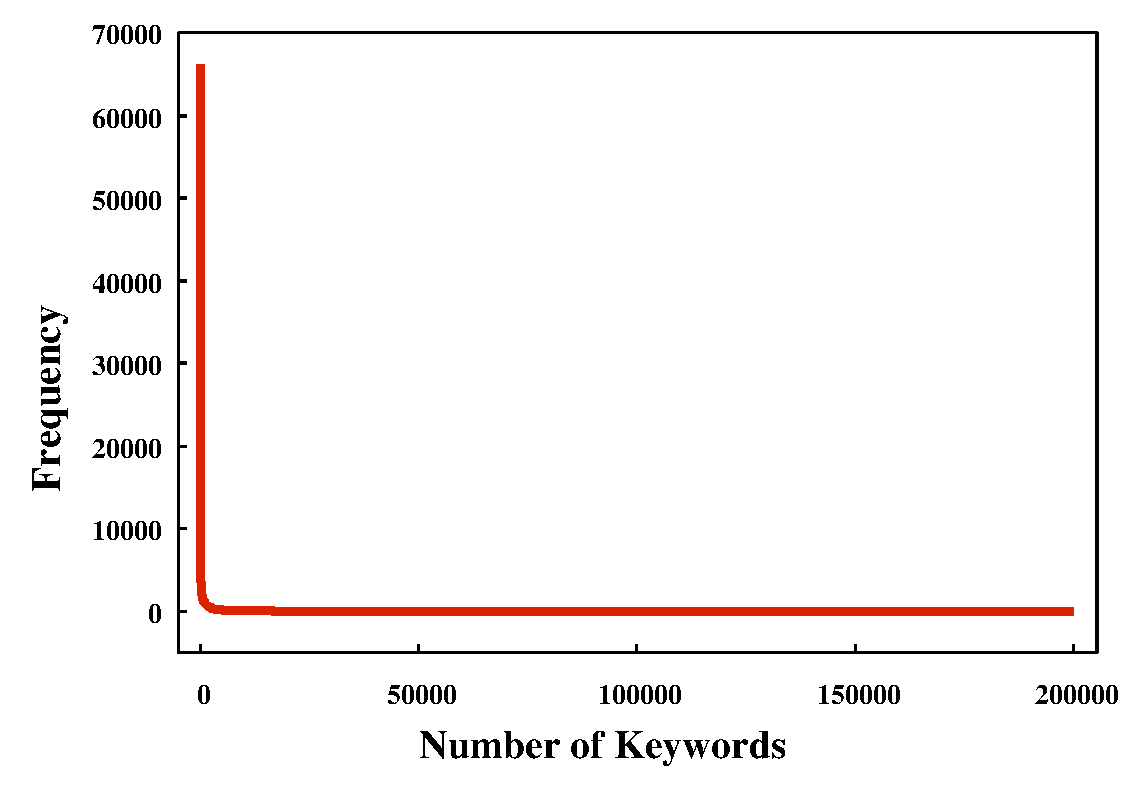
\includegraphics[width=7cm]{visuals/LongTail.eps} }}
  \qquad
  \subfloat[Log-Log distribution of AOL search query logs]{{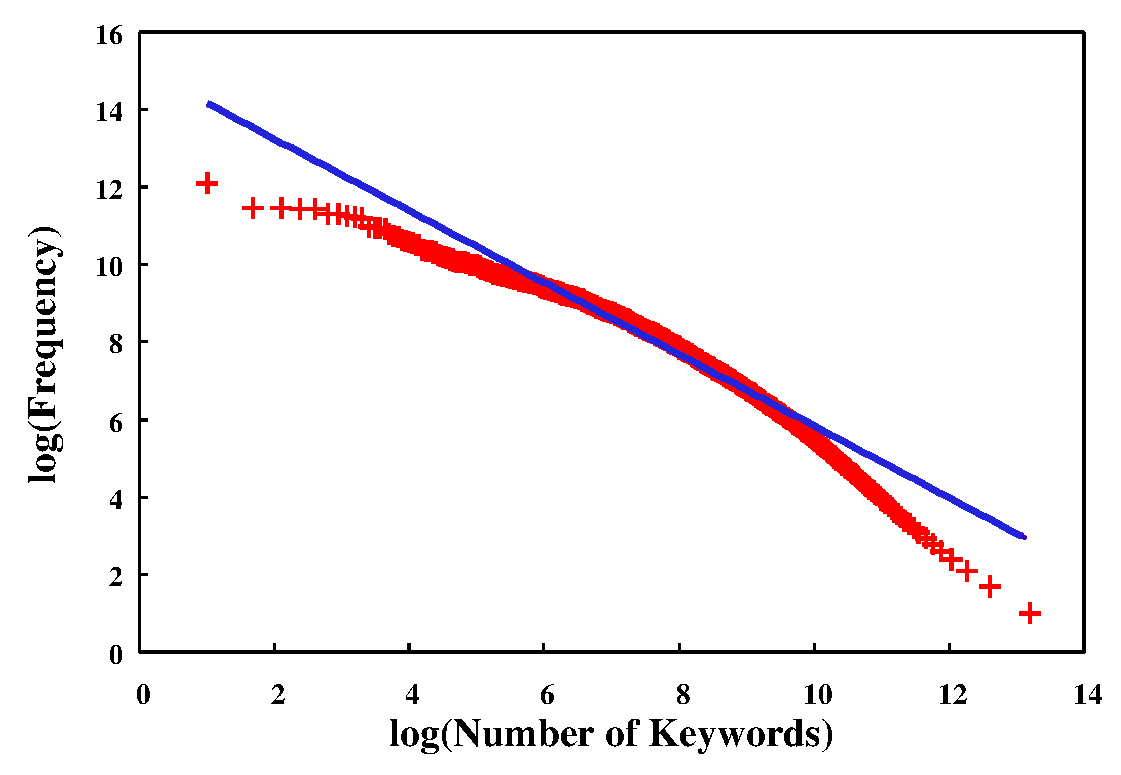
\includegraphics[width=7cm]{visuals/LogLogFinal.eps} }}
  \caption{Long tail distribution of AOL search query logs with a short head of frequent keywords and long tail of infrequent keywords is shown in (a). Log-Log distribution of AOL search query logs in shown in (b). Log-Log distribution of a perfect long tail should align to a straight line.}
  \label{longTail}
\end{figure}


\section{Overview of Proposed Approaches}
In this thesis, we have studied the issue of under-utilization of ad space of tail queries in sponsored search. We propose that advertisers should bid upon high levels concepts instead of keywords in the ad space auctions. In the first approach, we consider that the concepts are organized in a two level taxonomy. In the second approach, we propose a generalized approach by considering organization of concepts in a multi-level taxonomy. 


In the first approach, we have investigated bidding on concepts using a two level taxonomy.  Advertisers can bid only on the first level and sets of children nodes of the bid nodes are allocated to the advertisers. The notion of coverage patterns has been employed to form these groups of children nodes. In the literature, a coverage pattern has been defined as a set of items which \textit{covers} a minimum fraction of transactions and has a maximal \textit{overlap} of transactions within the items in the pattern. To extract coverage patterns, we utilize the notion of search sessions by considering the queries typed in the same session as a transaction. We further transform each transaction by replacing each query with the first and second level nodes as per the bidding taxonomy. Thus, each transaction is translated into taxonomy nodes. Coverage patterns are extracted from these taxonomy-based search transactions. The extracted coverage patterns help in identifying mutually exclusive sets of taxonomy nodes which ensure certain coverage along with a maximum overlap of transactions, thereby reducing the repetition of nodes in the same transaction. An approximate matching is performed between the extracted coverage patterns and advertising demands. Using the matching, we have defined an end-to-end architecture to allocate ads to an incoming query. Experiments on the real world dataset of AOL search query logs show that the proposed approach can help in exploiting ad space of long tail queries.

In the second approach, we generalize bidding in ad space auctions from a two level taxonomy to a multi-level taxonomy. Advertisers are free to bid on any node in the taxonomy. Bidding on any node in the taxonomy provides more flexibility to the advertisers to target potential consumers. During ad campaign creation, an advertiser is shown a taxonomy based on his/her ad content and is asked to select a node which he/she deems to be most relevant to the product being advertised. A set of children nodes of the bid node is allocated to the advertisers, similar to the first approach. However, each node in the taxonomy is composed of its descendants. For example, if we consider a node \textit{Shopping}, it will be composed of children nodes like \textit{Books, Fashion} and \textit{Electronics}. Thus, each transaction which consists of \textit{Books} will also consist of the node \textit{Shopping} as that transaction also belongs to \textit{Shopping}. If we model each search session as a transaction of taxonomy nodes, as proposed in the first approach, and mine coverage patterns, we will get coverage patterns where items are dependent upon each other. Thus the flat model of coverage patterns cannot be employed to allocate children nodes of bidden nodes to advertisers. We extend the model of coverage patterns by proposing the notion of \textit{level-wise coverage patterns} which takes a taxonomy and search query logs as input and outputs coverage patterns amongst items which are at the same level in the taxonomy. Thus, the notion of level-wise coverage patterns helps in resolving the interdependence of nodes in coverage patterns. Using the notion of \textit{level-wise coverage patterns} and \textit{bidding on high level concepts through a multi-level taxonomy}, we propose an end-to-end framework which takes search query logs, bidding taxonomy and advertising demands as inputs and allocates advertisements to an incoming query. Experiments results on AOL search query logs show that the proposed approach can help in better utilization of space for sponsored search.


In both approaches, we propose to bid upon concepts instead of keywords in sponsored search auctions. The notion of concept-based bidding will result in capitalization of ad space of the tail queries as each concept will be composed of both head and tail keywords. Hence, each keyword would be considered for bidding based on its relevancy rather than frequency.


\section{Contributions of Thesis}
The contributions of the thesis are as follows:

\begin{enumerate}[label=(\roman*).]
\item \textbf{An approach to bid on concepts in sponsored search:} In this thesis, we propose to sell high level concepts (using a two level taxonomy) in the ad space auctions instead of individual keywords. We argue that high order logical concepts are composed of head and tail keywords alike and bidding on such concepts would result in the capitalization of ad space of search keywords irrespective of their frequency.

\item \textbf{An approach to bid on a taxonomy in sponsored search:} In this approach, we propose to use a multi-level taxonomy for ad space auctions to provide more flexibility to the advertisers to target potential consumers.

\item \textbf{Algorithms and optimization objectives:} Algorithms and optimization objectives for the above approaches are also a part of this thesis.

\item \textbf{Experimental results:} Experiments have been conducted on a real world dataset of AOL search query logs to compare the performance of proposed approaches with the traditional sponsored search approach.

\item \textbf{Literature survey:} The thesis provide a detailed survey on long tail advertising in sponsored search and on coverage patterns.

\end{enumerate}

\section{Organization of Thesis}

The rest of the thesis is organized as follows:
\begin{enumerate}[label=(\roman*).]

\item In Chapter 2, the Related Work for the sponsored search mechanisms and long tail advertising has been covered. We also discuss related literature of coverage patterns, as coverage patterns constitute to be a main part of the proposed approaches.

\item In Chapter 3, we discuss the sponsored search architecture and an overview of coverage patterns.

\item In Chapter 4, the first approach for long tail advertising in sponsored search has been proposed where we propose to extend the model of bidding on keywords in sponsored search to bidding on higher level concepts through a two level taxonomy.

\item In Chapter 5, the second approach for long tail advertising in sponsored search  has been proposed where we generalize the first approach to use multi-level taxonomy during ad space auctions.

\item In Chapter 6, we discuss conclusions and directions to future work.

\end{enumerate}

